%!TEX root = thesis.tex

\appendix

\chapter{Images}

\begin{figure}[tb]
\begin{center}
\subfloat[input frame]{\label{fig:pipe_input}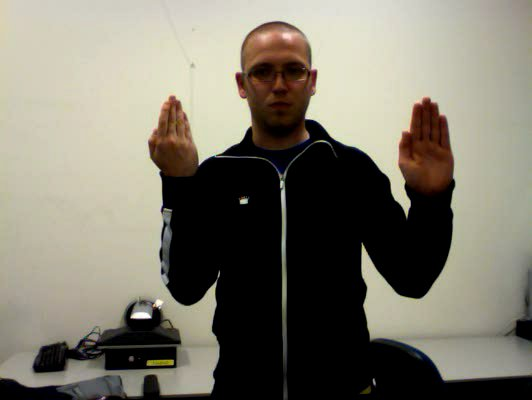
\includegraphics[width=0.3\linewidth]{figures/pipeline/input.jpg}}
\hspace{0.03\linewidth}
\subfloat[hue channel]{\label{fig:hue2}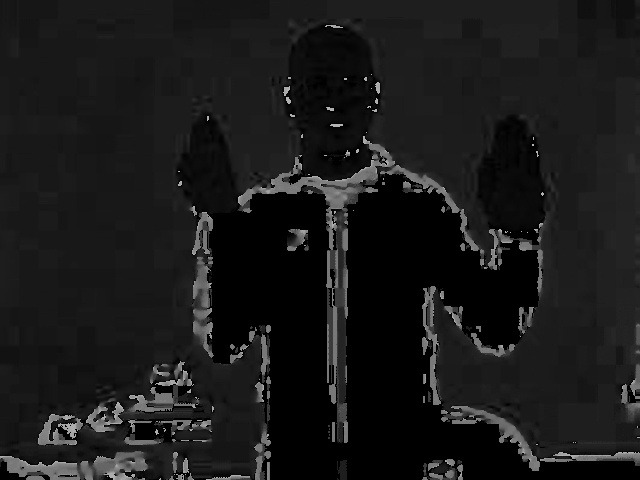
\includegraphics[width=0.3\linewidth]{figures/pipeline/hue.jpg}}
\hspace{0.03\linewidth}
\subfloat[saturation channel]{\label{fig:saturation2}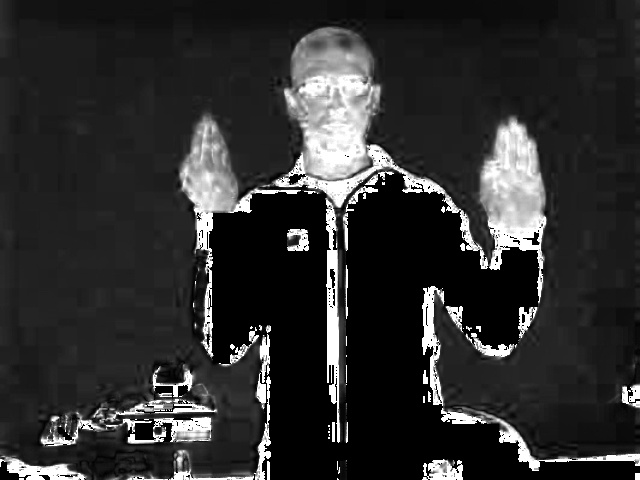
\includegraphics[width=0.3\linewidth]{figures/pipeline/saturation.jpg}}
\hspace{0.03\linewidth}
\subfloat[value channel]{\label{fig:value2}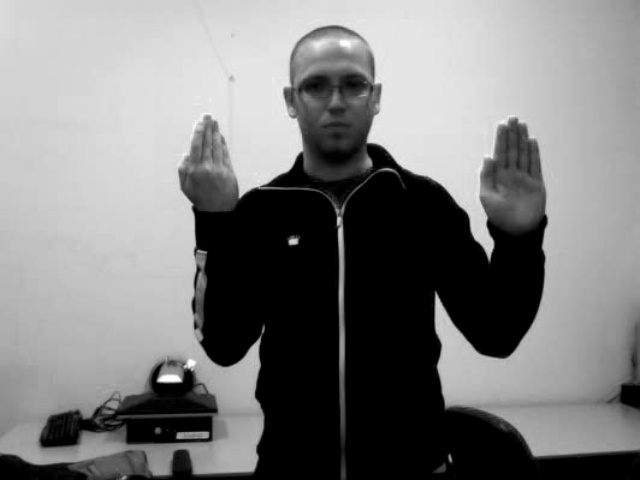
\includegraphics[width=0.3\linewidth]{figures/pipeline/value.jpg}}
\hspace{0.03\linewidth}
\subfloat[face detection]{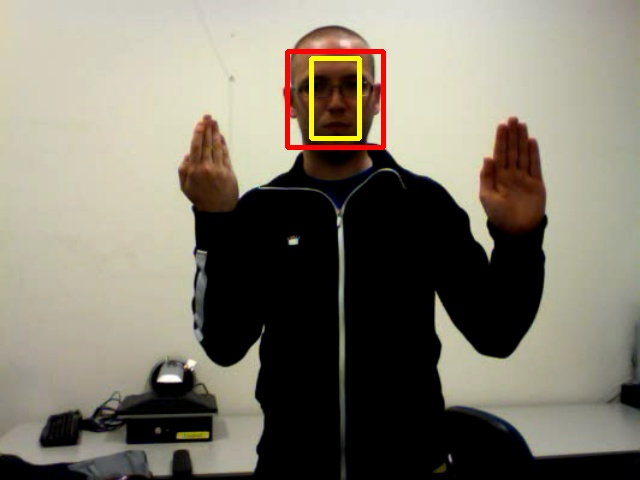
\includegraphics[width=0.3\linewidth]{figures/pipeline/detected.jpg}}
\hspace{0.03\linewidth}
\subfloat[Face color histogram]{\label{fig:pipe_hist}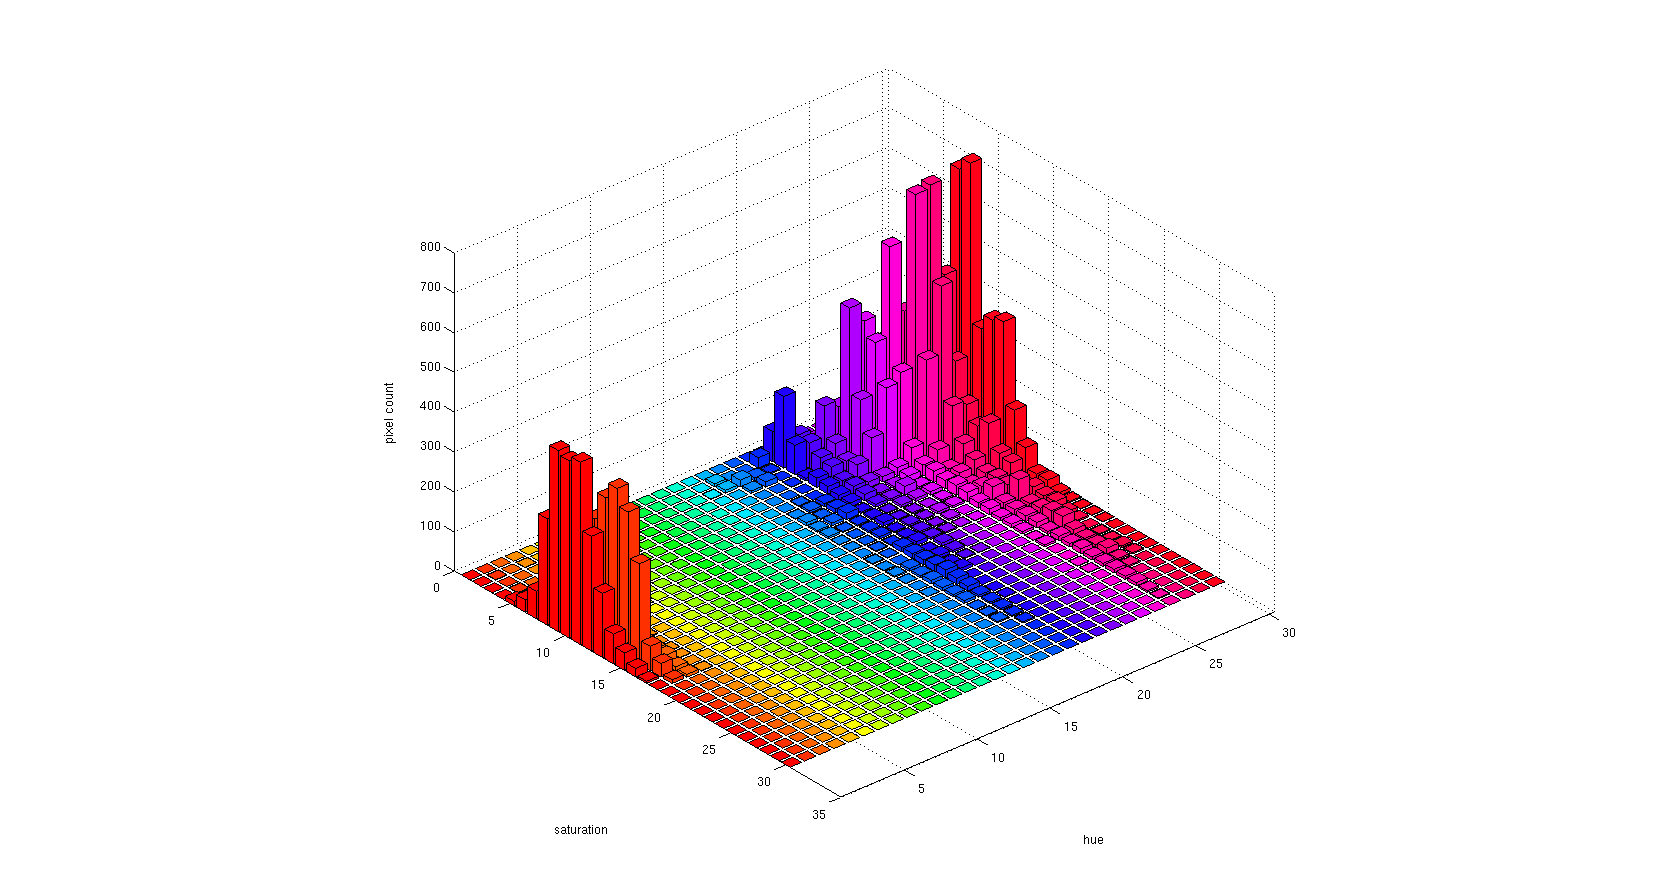
\includegraphics[width=0.3\linewidth]{figures/pipeline/histogram.png}}
\hspace{0.03\linewidth}
\subfloat[Backprojection]{\label{fig:pipe_bp}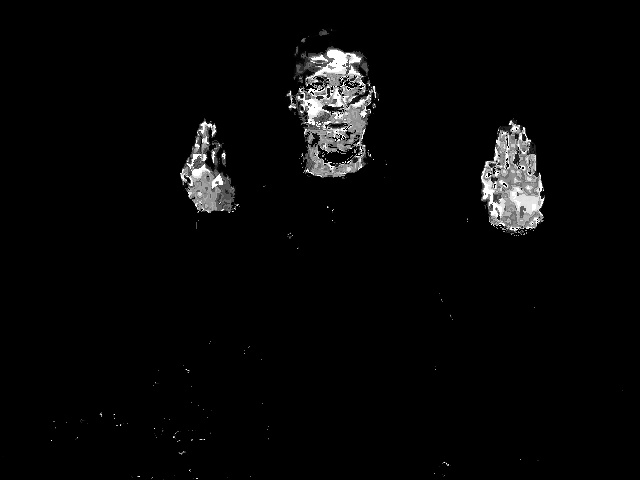
\includegraphics[width=0.3\linewidth]{figures/pipeline/backproject.jpg}}
\hspace{0.03\linewidth}
\subfloat[Gaussian smooth]{\label{fig:pipe_blur}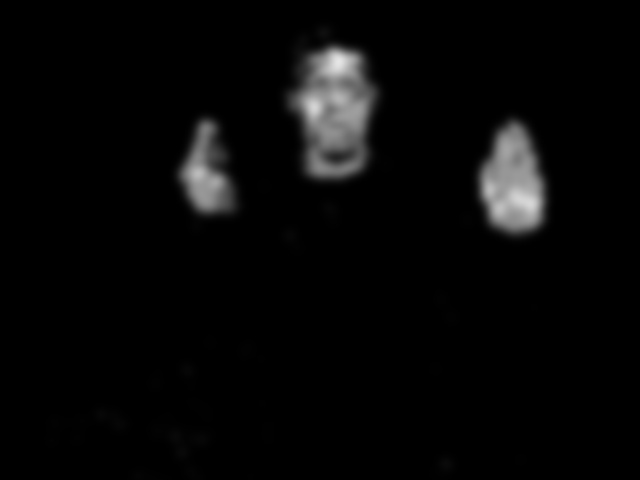
\includegraphics[width=0.3\linewidth]{figures/pipeline/blurred.jpg}}
\hspace{0.03\linewidth}
\subfloat[Thresholded binary image]{\label{fig:pipe_th}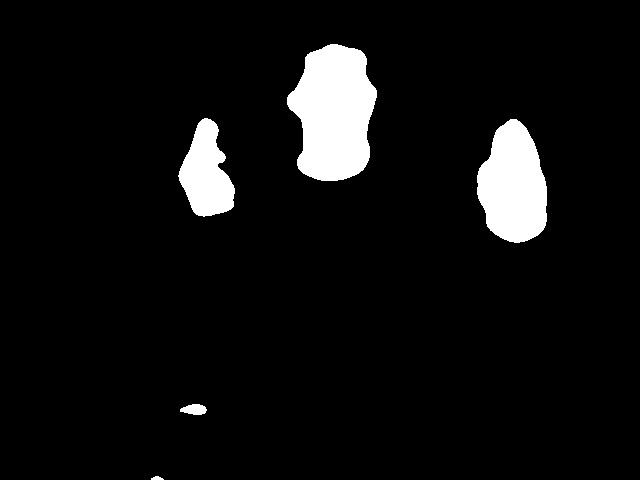
\includegraphics[width=0.3\linewidth]{figures/pipeline/thresholded.jpg}}
\hspace{0.03\linewidth}
\subfloat[Morpholoical close]{\label{fig:pipe_close}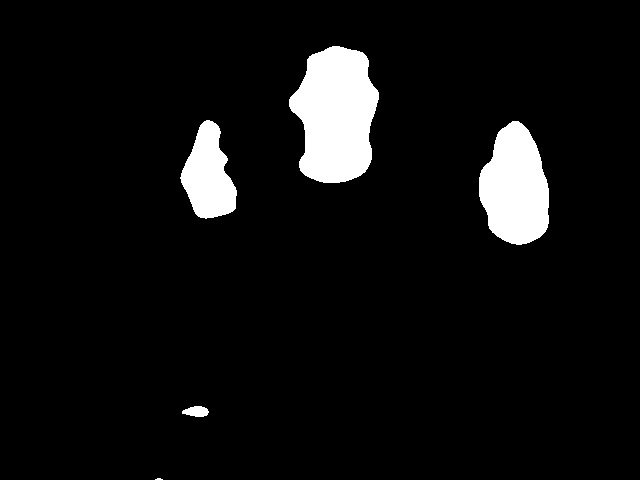
\includegraphics[width=0.3\linewidth]{figures/pipeline/closed.jpg}}
\hspace{0.03\linewidth}
\subfloat[Blob labeling]{\label{fig:pipe_cont}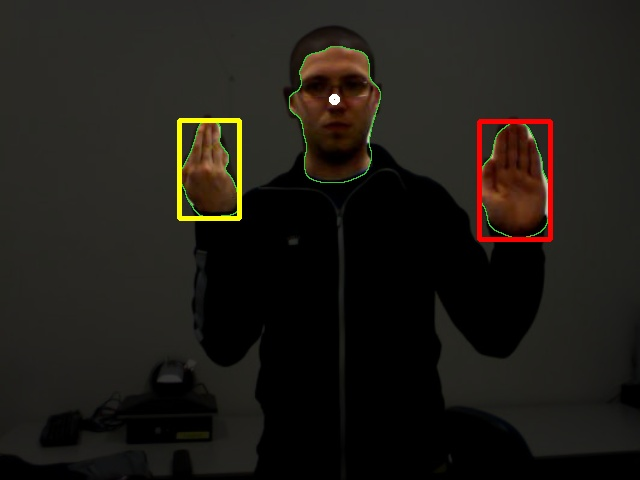
\includegraphics[width=0.3\linewidth]{figures/pipeline/contours.jpg}}
\end{center}
\caption{The complete hand pose detection pipeline}
\label{fig:pipeline}
\end{figure}


\renewcommand{\thesubfigure}{\thefigure.\roman{subfigure}}
\begin{figure}[tb]
\begin{center}
\subfloat[Do1]{\label{fig:hand_0}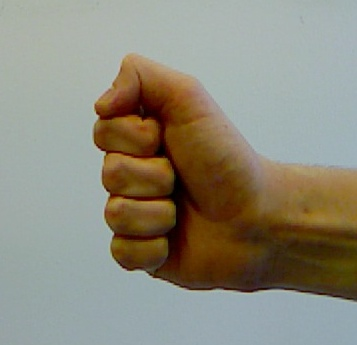
\includegraphics[width=0.2\linewidth,height=0.15\linewidth]{figures/examples/0.jpg}}
\hspace{0.03\linewidth}
\subfloat[Di1]{\label{fig:hand_1}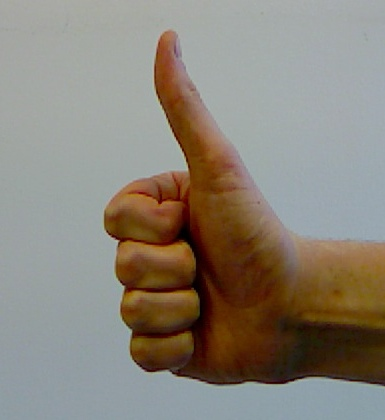
\includegraphics[width=0.2\linewidth,height=0.15\linewidth]{figures/examples/1.jpg}}
\hspace{0.03\linewidth}
\subfloat[Re1]{\label{fig:hand_2}
\includegraphics[width=0.2\linewidth,height=0.15\linewidth]{figures/examples/2.jpg}}
\hspace{0.03\linewidth}
\subfloat[Ri1]{\label{fig:hand_3}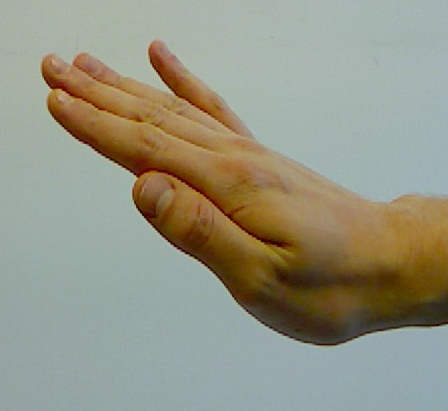
\includegraphics[width=0.2\linewidth,height=0.15\linewidth]{figures/examples/3.jpg}}
\hspace{0.03\linewidth}
\subfloat[Mi1]{\label{fig:hand_4}
\includegraphics[width=0.2\linewidth,height=0.15\linewidth]{figures/examples/4.jpg}}
\hspace{0.03\linewidth}
\subfloat[Fa1]{\label{fig:hand_5}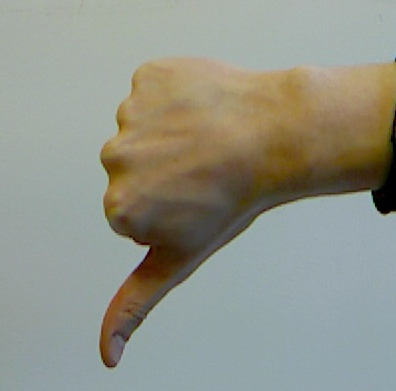
\includegraphics[width=0.2\linewidth,height=0.15\linewidth]{figures/examples/5.jpg}}
\hspace{0.03\linewidth}
\subfloat[Fi1]{\label{fig:hand_6}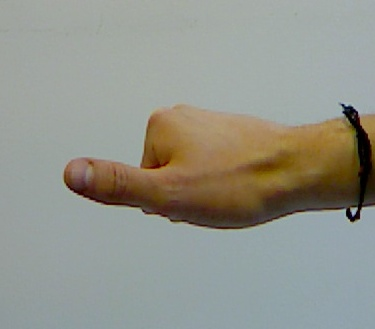
\includegraphics[width=0.2\linewidth,height=0.15\linewidth]{figures/examples/6.jpg}}
\hspace{0.03\linewidth}
\subfloat[Sol1]{\label{fig:hand_7}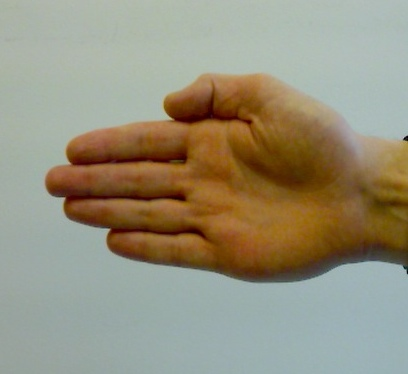
\includegraphics[width=0.2\linewidth,height=0.15\linewidth]{figures/examples/7.jpg}}
\hspace{0.03\linewidth}
\subfloat[Si1]{\label{fig:hand_8}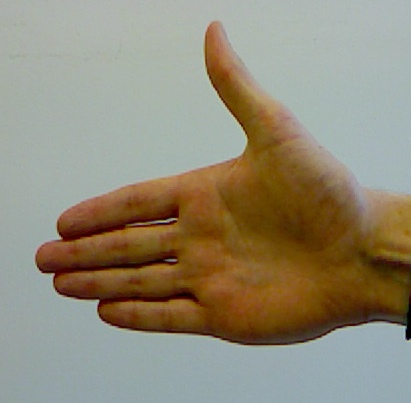
\includegraphics[width=0.2\linewidth,height=0.15\linewidth]{figures/examples/8.jpg}}
\hspace{0.03\linewidth}
\subfloat[La1]{\label{fig:hand_9}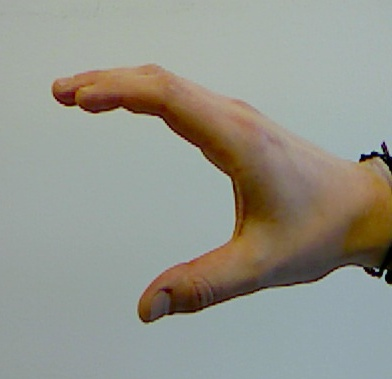
\includegraphics[width=0.2\linewidth,height=0.15\linewidth]{figures/examples/9.jpg}}
\hspace{0.03\linewidth}
\subfloat[Li1]{\label{fig:hand_10}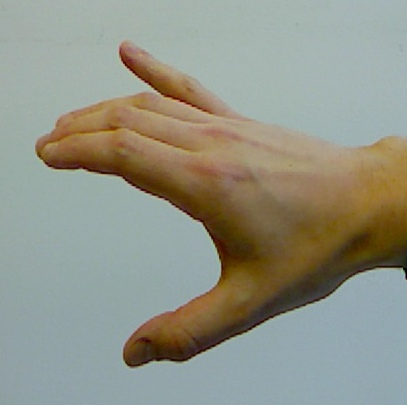
\includegraphics[width=0.2\linewidth,height=0.15\linewidth]{figures/examples/10.jpg}}
\hspace{0.03\linewidth}
\subfloat[Ti1]{\label{fig:hand_11}
\includegraphics[width=0.2\linewidth,height=0.15\linewidth]{figures/examples/11.jpg}}
\hspace{0.03\linewidth}
\subfloat[Do2]{\label{fig:hand_12}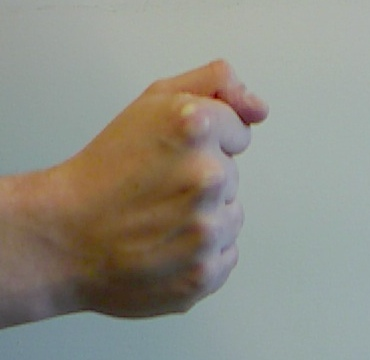
\includegraphics[width=0.2\linewidth,height=0.15\linewidth]{figures/examples/12.jpg}}
\hspace{0.03\linewidth}
\subfloat[Di2]{\label{fig:hand_13}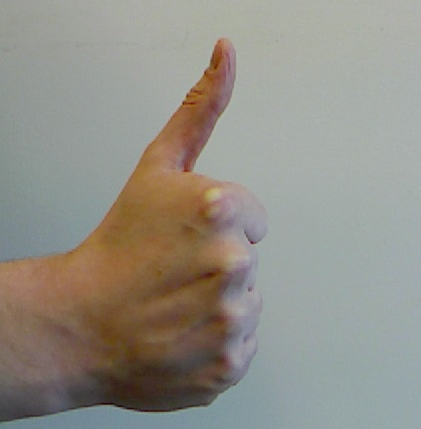
\includegraphics[width=0.2\linewidth,height=0.15\linewidth]{figures/examples/13.jpg}}
\hspace{0.03\linewidth}
\subfloat[Re2]{\label{fig:hand_14}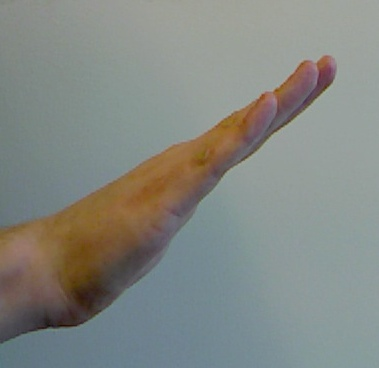
\includegraphics[width=0.2\linewidth,height=0.15\linewidth]{figures/examples/14.jpg}}
\hspace{0.03\linewidth}
\subfloat[Ri2]{\label{fig:hand_15}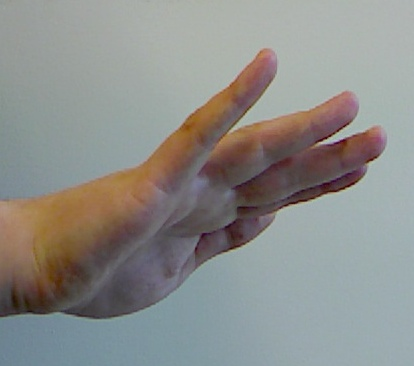
\includegraphics[width=0.2\linewidth,height=0.15\linewidth]{figures/examples/15.jpg}}
\hspace{0.03\linewidth}
\subfloat[Mi2]{\label{fig:hand_16}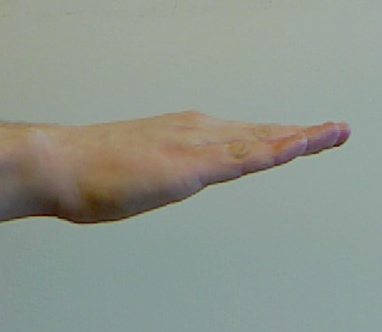
\includegraphics[width=0.2\linewidth,height=0.15\linewidth]{figures/examples/16.jpg}}
\hspace{0.03\linewidth}
\subfloat[Fa2]{\label{fig:hand_17}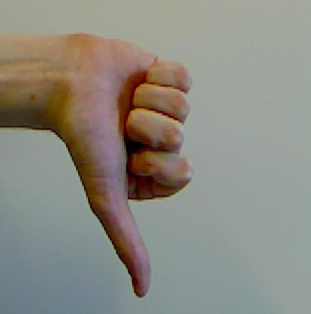
\includegraphics[width=0.2\linewidth,height=0.15\linewidth]{figures/examples/17.jpg}}
\hspace{0.03\linewidth}
\subfloat[Fi2]{\label{fig:hand_18}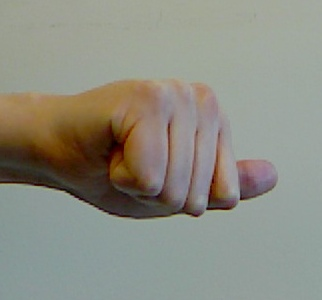
\includegraphics[width=0.2\linewidth,height=0.15\linewidth]{figures/examples/18.jpg}}
\hspace{0.03\linewidth}
\subfloat[So2l]{\label{fig:hand_19}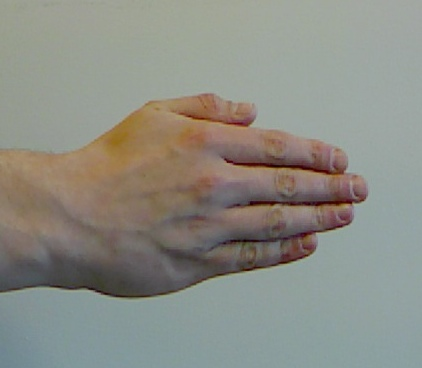
\includegraphics[width=0.2\linewidth,height=0.15\linewidth]{figures/examples/19.jpg}}
\hspace{0.03\linewidth}
\subfloat[Si2]{\label{fig:hand_20}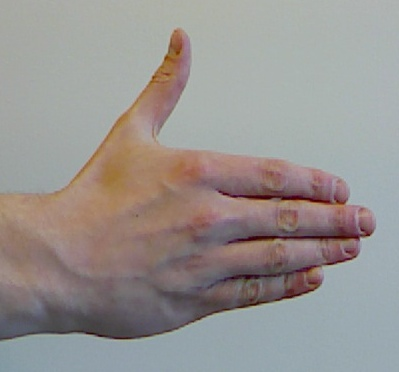
\includegraphics[width=0.2\linewidth,height=0.15\linewidth]{figures/examples/20.jpg}}
\hspace{0.03\linewidth}
\subfloat[La2]{\label{fig:hand_21}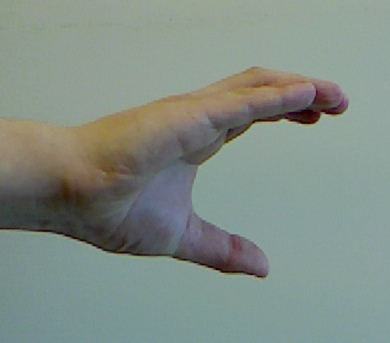
\includegraphics[width=0.2\linewidth,height=0.15\linewidth]{figures/examples/21.jpg}}
\hspace{0.03\linewidth}
\subfloat[Li2]{\label{fig:hand_22}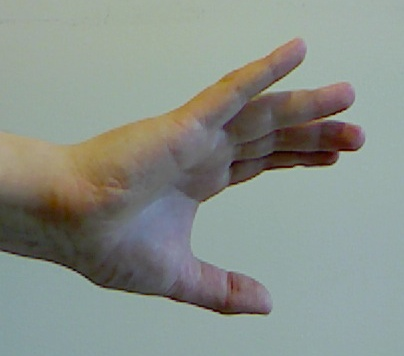
\includegraphics[width=0.2\linewidth,height=0.15\linewidth]{figures/examples/22.jpg}}
\hspace{0.03\linewidth}
\subfloat[Ti2]{\label{fig:hand_23}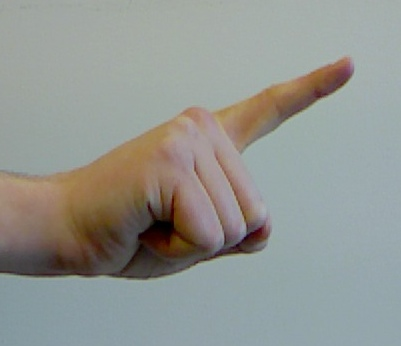
\includegraphics[width=0.2\linewidth,height=0.15\linewidth]{figures/examples/23.jpg}}
\hspace{0.03\linewidth}
\subfloat[I]{\label{fig:hand_24}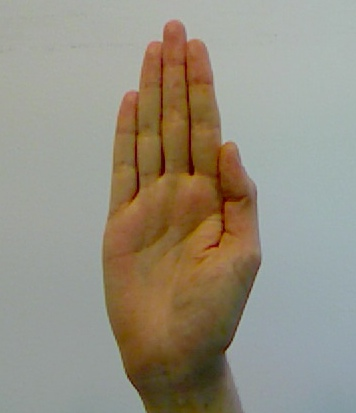
\includegraphics[width=0.2\linewidth,height=0.15\linewidth]{figures/examples/24.jpg}}
\hspace{0.03\linewidth}
\subfloat[I]{\label{fig:hand_25}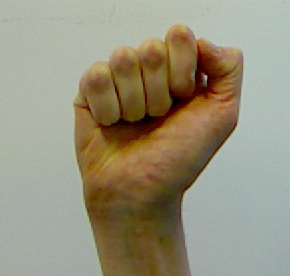
\includegraphics[width=0.2\linewidth,height=0.15\linewidth]{figures/examples/25.jpg}}
\hspace{0.03\linewidth}
\subfloat[III]{\label{fig:hand_26}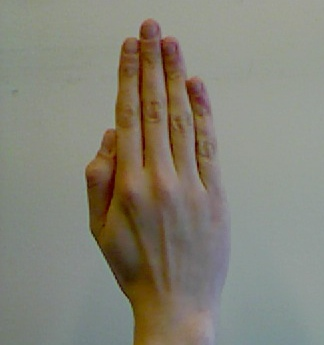
\includegraphics[width=0.2\linewidth,height=0.15\linewidth]{figures/examples/26.jpg}}
\hspace{0.03\linewidth}
\subfloat[IV]{\label{fig:hand_27}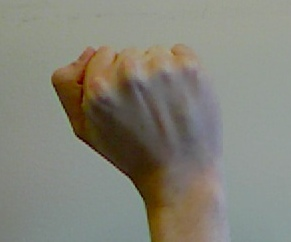
\includegraphics[width=0.2\linewidth,height=0.15\linewidth]{figures/examples/27.jpg}}
\end{center}
\caption{The example hand poses a shown to the test subjects}
\label{fig:hands}
\end{figure}


\begin{figure}[tb]
\begin{center}
\subfloat[Do1]{\label{fig:gijs5_0}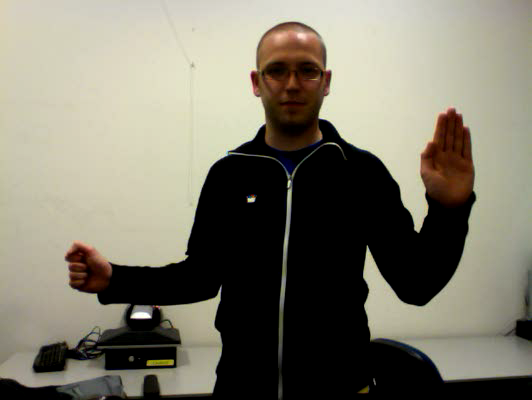
\includegraphics[width=0.2\linewidth,height=0.15\linewidth]{figures/gijs5/0.png}}
\hspace{0.03\linewidth}
\subfloat[Di1]{\label{fig:gijs5_1}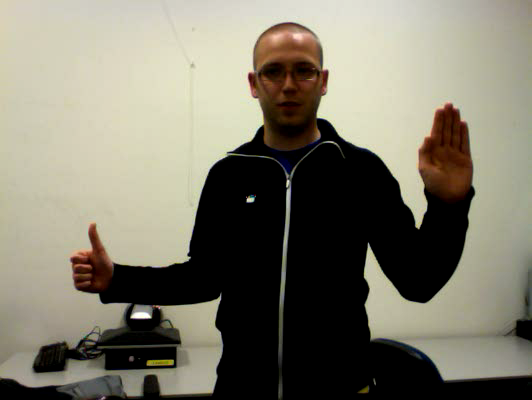
\includegraphics[width=0.2\linewidth,height=0.15\linewidth]{figures/gijs5/1.png}}
\hspace{0.03\linewidth}
\subfloat[Re1]{\label{fig:gijs5_2}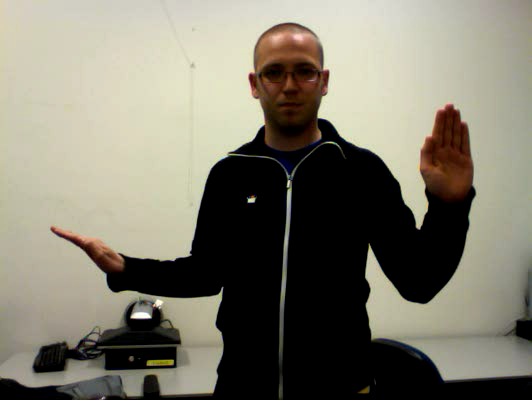
\includegraphics[width=0.2\linewidth,height=0.15\linewidth]{figures/gijs5/2.png}}
\hspace{0.03\linewidth}
\subfloat[Ri1]{\label{fig:gijs5_3}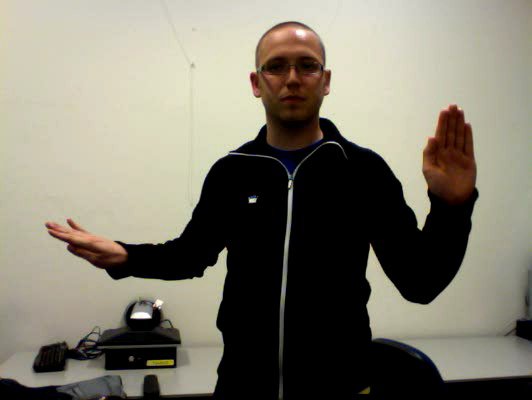
\includegraphics[width=0.2\linewidth,height=0.15\linewidth]{figures/gijs5/3.png}}
\hspace{0.03\linewidth}
\subfloat[Mi1]{\label{fig:gijs5_4}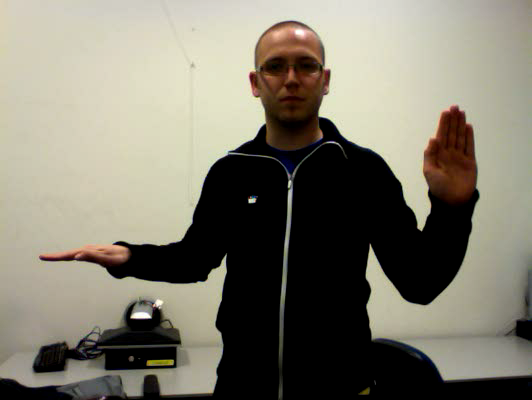
\includegraphics[width=0.2\linewidth,height=0.15\linewidth]{figures/gijs5/4.png}}
\hspace{0.03\linewidth}
\subfloat[Fa1]{\label{fig:gijs5_5}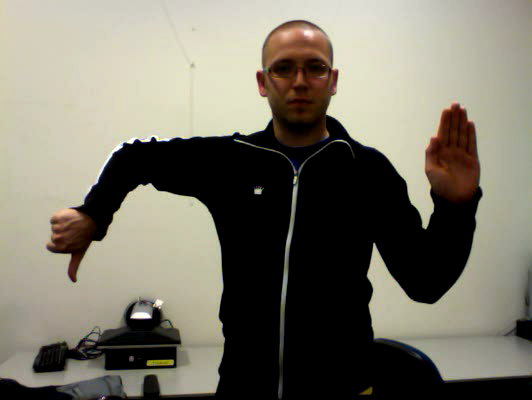
\includegraphics[width=0.2\linewidth,height=0.15\linewidth]{figures/gijs5/5.png}}
\hspace{0.03\linewidth}
\subfloat[Fi1]{\label{fig:gijs5_6}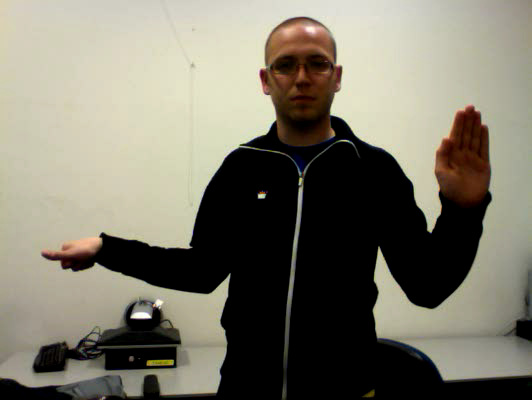
\includegraphics[width=0.2\linewidth,height=0.15\linewidth]{figures/gijs5/6.png}}
\hspace{0.03\linewidth}
\subfloat[Sol1]{\label{fig:gijs5_7}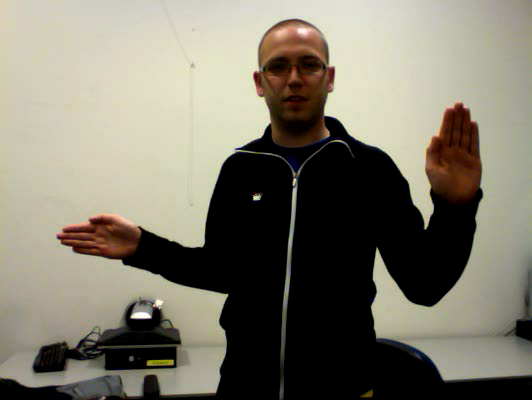
\includegraphics[width=0.2\linewidth,height=0.15\linewidth]{figures/gijs5/7.png}}
\hspace{0.03\linewidth}
\subfloat[Si1]{\label{fig:gijs5_8}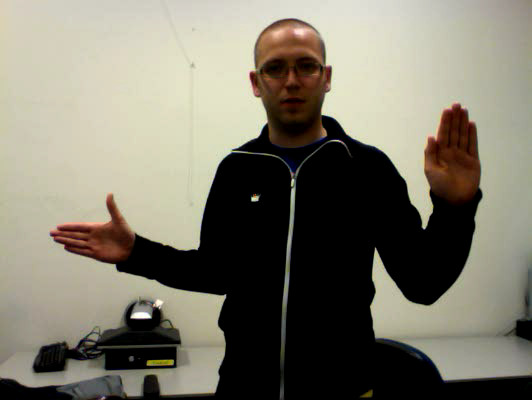
\includegraphics[width=0.2\linewidth,height=0.15\linewidth]{figures/gijs5/8.png}}
\hspace{0.03\linewidth}
\subfloat[La1]{\label{fig:gijs5_9}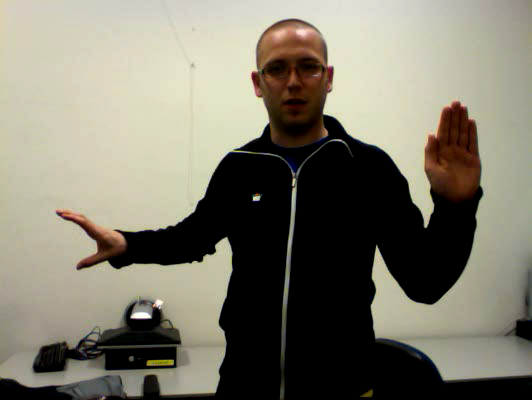
\includegraphics[width=0.2\linewidth,height=0.15\linewidth]{figures/gijs5/9.png}}
\hspace{0.03\linewidth}
\subfloat[Li1]{\label{fig:gijs5_10}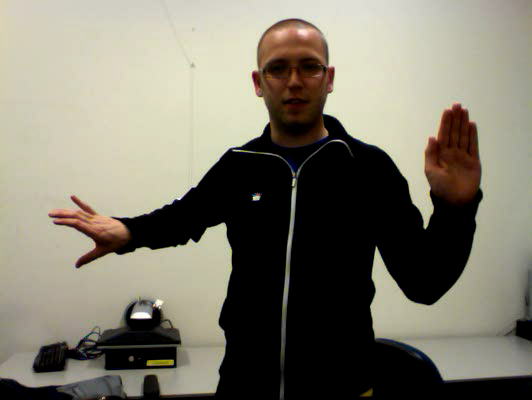
\includegraphics[width=0.2\linewidth,height=0.15\linewidth]{figures/gijs5/10.png}}
\hspace{0.03\linewidth}
\subfloat[Ti1]{\label{fig:gijs5_11}\includegraphics[width=0.2\linewidth,height=0.15\linewidth]{figures/gijs5/11.png}}
\hspace{0.03\linewidth}
\subfloat[Do2]{\label{fig:gijs5_12}\includegraphics[width=0.2\linewidth,height=0.15\linewidth]{figures/gijs5/12.png}}
\hspace{0.03\linewidth}
\subfloat[Di2]{\label{fig:gijs5_13}\includegraphics[width=0.2\linewidth,height=0.15\linewidth]{figures/gijs5/13.png}}
\hspace{0.03\linewidth}
\subfloat[Re2]{\label{fig:gijs5_14}\includegraphics[width=0.2\linewidth,height=0.15\linewidth]{figures/gijs5/14.png}}
\hspace{0.03\linewidth}
\subfloat[Ri2]{\label{fig:gijs5_15}\includegraphics[width=0.2\linewidth,height=0.15\linewidth]{figures/gijs5/15.png}}
\hspace{0.03\linewidth}
\subfloat[Mi2]{\label{fig:gijs5_16}\includegraphics[width=0.2\linewidth,height=0.15\linewidth]{figures/gijs5/16.png}}
\hspace{0.03\linewidth}
\subfloat[Fa2]{\label{fig:gijs5_17}\includegraphics[width=0.2\linewidth,height=0.15\linewidth]{figures/gijs5/17.png}}
\hspace{0.03\linewidth}
\subfloat[Fi2]{\label{fig:gijs5_18}\includegraphics[width=0.2\linewidth,height=0.15\linewidth]{figures/gijs5/18.png}}
\hspace{0.03\linewidth}
\subfloat[Sol2]{\label{fig:gijs5_19}\includegraphics[width=0.2\linewidth,height=0.15\linewidth]{figures/gijs5/19.png}}
\hspace{0.03\linewidth}
\subfloat[Si2]{\label{fig:gijs5_20}\includegraphics[width=0.2\linewidth,height=0.15\linewidth]{figures/gijs5/20.png}}
\hspace{0.03\linewidth}
\subfloat[La2]{\label{fig:gijs5_21}\includegraphics[width=0.2\linewidth,height=0.15\linewidth]{figures/gijs5/21.png}}
\hspace{0.03\linewidth}
\subfloat[Li2]{\label{fig:gijs5_22}\includegraphics[width=0.2\linewidth,height=0.15\linewidth]{figures/gijs5/22.png}}
\hspace{0.03\linewidth}
\subfloat[Ti2]{\label{fig:gijs5_23}\includegraphics[width=0.2\linewidth,height=0.15\linewidth]{figures/gijs5/23.png}}
\hspace{0.03\linewidth}
\subfloat[I]{\label{fig:gijs5_24}\includegraphics[width=0.2\linewidth,height=0.15\linewidth]{figures/gijs5/24.png}}
\hspace{0.03\linewidth}
\subfloat[II]{\label{fig:gijs5_25}\includegraphics[width=0.2\linewidth,height=0.15\linewidth]{figures/gijs5/25.png}}
\hspace{0.03\linewidth}
\subfloat[III]{\label{fig:gijs5_26}\includegraphics[width=0.2\linewidth,height=0.15\linewidth]{figures/gijs5/26.png}}
\hspace{0.03\linewidth}
\subfloat[IV]{\label{fig:gijs5_27}\includegraphics[width=0.2\linewidth,height=0.15\linewidth]{figures/gijs5/27.png}}
\end{center}
\caption{The labeled frames of a movie from the dataset}
\label{fig:gijs5}
\end{figure}



\begin{figure}[tb]
\begin{center}
\subfloat[Do1]{\label{fig:gijs5_cutout_0}\includegraphics[width=0.2\linewidth,height=0.15\linewidth]{figures/gijs5_cutout/0.jpg}}
\hspace{0.03\linewidth}
\subfloat[Di1]{\label{fig:gijs5_cutout_1}\includegraphics[width=0.2\linewidth,height=0.15\linewidth]{figures/gijs5_cutout/1.jpg}}
\hspace{0.03\linewidth}
\subfloat[Re1]{\label{fig:gijs5_cutout_2}\includegraphics[width=0.2\linewidth,height=0.15\linewidth]{figures/gijs5_cutout/2.jpg}}
\hspace{0.03\linewidth}
\subfloat[Ri1]{\label{fig:gijs5_cutout_3}\includegraphics[width=0.2\linewidth,height=0.15\linewidth]{figures/gijs5_cutout/3.jpg}}
\hspace{0.03\linewidth}
\subfloat[Mi1]{\label{fig:gijs5_cutout_4}\includegraphics[width=0.2\linewidth,height=0.15\linewidth]{figures/gijs5_cutout/4.jpg}}
\hspace{0.03\linewidth}
\subfloat[Fa1]{\label{fig:gijs5_cutout_5}\includegraphics[width=0.2\linewidth,height=0.15\linewidth]{figures/gijs5_cutout/5.jpg}}
\hspace{0.03\linewidth}
\subfloat[Fi1]{\label{fig:gijs5_cutout_6}\includegraphics[width=0.2\linewidth,height=0.15\linewidth]{figures/gijs5_cutout/6.jpg}}
\hspace{0.03\linewidth}
\subfloat[Sol1]{\label{fig:gijs5_cutout_7}\includegraphics[width=0.2\linewidth,height=0.15\linewidth]{figures/gijs5_cutout/7.jpg}}
\hspace{0.03\linewidth}
\subfloat[Si1]{\label{fig:gijs5_cutout_8}\includegraphics[width=0.2\linewidth,height=0.15\linewidth]{figures/gijs5_cutout/8.jpg}}
\hspace{0.03\linewidth}
\subfloat[La1]{\label{fig:gijs5_cutout_9}\includegraphics[width=0.2\linewidth,height=0.15\linewidth]{figures/gijs5_cutout/9.jpg}}
\hspace{0.03\linewidth}
\subfloat[Li1]{\label{fig:gijs5_cutout_10}\includegraphics[width=0.2\linewidth,height=0.15\linewidth]{figures/gijs5_cutout/10.jpg}}
\hspace{0.03\linewidth}
\subfloat[Ti1]{\label{fig:gijs5_cutout_11}\includegraphics[width=0.2\linewidth,height=0.15\linewidth]{figures/gijs5_cutout/11.jpg}}
\hspace{0.03\linewidth}
\subfloat[Do2]{\label{fig:gijs5_cutout_12}\includegraphics[width=0.2\linewidth,height=0.15\linewidth]{figures/gijs5_cutout/12.jpg}}
\hspace{0.03\linewidth}
\subfloat[Di2]{\label{fig:gijs5_cutout_13}\includegraphics[width=0.2\linewidth,height=0.15\linewidth]{figures/gijs5_cutout/13.jpg}}
\hspace{0.03\linewidth}
\subfloat[Re2]{\label{fig:gijs5_cutout_14}\includegraphics[width=0.2\linewidth,height=0.15\linewidth]{figures/gijs5_cutout/14.jpg}}
\hspace{0.03\linewidth}
\subfloat[Ri2]{\label{fig:gijs5_cutout_15}\includegraphics[width=0.2\linewidth,height=0.15\linewidth]{figures/gijs5_cutout/15.jpg}}
\hspace{0.03\linewidth}
\subfloat[Mi2]{\label{fig:gijs5_cutout_16}\includegraphics[width=0.2\linewidth,height=0.15\linewidth]{figures/gijs5_cutout/16.jpg}}
\hspace{0.03\linewidth}
\subfloat[Fa2]{\label{fig:gijs5_cutout_17}\includegraphics[width=0.2\linewidth,height=0.15\linewidth]{figures/gijs5_cutout/17.jpg}}
\hspace{0.03\linewidth}
\subfloat[Fi2]{\label{fig:gijs5_cutout_18}\includegraphics[width=0.2\linewidth,height=0.15\linewidth]{figures/gijs5_cutout/18.jpg}}
\hspace{0.03\linewidth}
\subfloat[Sol2]{\label{fig:gijs5_cutout_19}\includegraphics[width=0.2\linewidth,height=0.15\linewidth]{figures/gijs5_cutout/19.jpg}}
\hspace{0.03\linewidth}
\subfloat[Si2]{\label{fig:gijs5_cutout_20}\includegraphics[width=0.2\linewidth,height=0.15\linewidth]{figures/gijs5_cutout/20.jpg}}
\hspace{0.03\linewidth}
\subfloat[La2]{\label{fig:gijs5_cutout_21}\includegraphics[width=0.2\linewidth,height=0.15\linewidth]{figures/gijs5_cutout/21.jpg}}
\hspace{0.03\linewidth}
\subfloat[Li2]{\label{fig:gijs5_cutout_22}\includegraphics[width=0.2\linewidth,height=0.15\linewidth]{figures/gijs5_cutout/22.jpg}}
\hspace{0.03\linewidth}
\subfloat[Ti2]{\label{fig:gijs5_cutout_23}\includegraphics[width=0.2\linewidth,height=0.15\linewidth]{figures/gijs5_cutout/23.jpg}}
\hspace{0.03\linewidth}
\subfloat[I]{\label{fig:gijs5_cutout_24}\includegraphics[width=0.2\linewidth,height=0.15\linewidth]{figures/gijs5_cutout/24.jpg}}
\hspace{0.03\linewidth}
\subfloat[II]{\label{fig:gijs5_cutout_25}\includegraphics[width=0.2\linewidth,height=0.15\linewidth]{figures/gijs5_cutout/25.jpg}}
\hspace{0.03\linewidth}
\subfloat[III]{\label{fig:gijs5_cutout_26}\includegraphics[width=0.2\linewidth,height=0.15\linewidth]{figures/gijs5_cutout/26.jpg}}
\hspace{0.03\linewidth}
\subfloat[IV]{\label{fig:gijs5_cutout_27}\includegraphics[width=0.2\linewidth,height=0.15\linewidth]{figures/gijs5_cutout/27.jpg}}
\end{center}
\caption{The hand windows, used for feature extraction}
\label{fig:gijs5_cutout}
\end{figure}

